\documentclass{standalone}

% graphics
\usepackage[usenames,dvipsnames]{xcolor}
\usepackage{tikz}
\usepackage{pgfplots}
\usepackage{siunitx}

\begin{document}

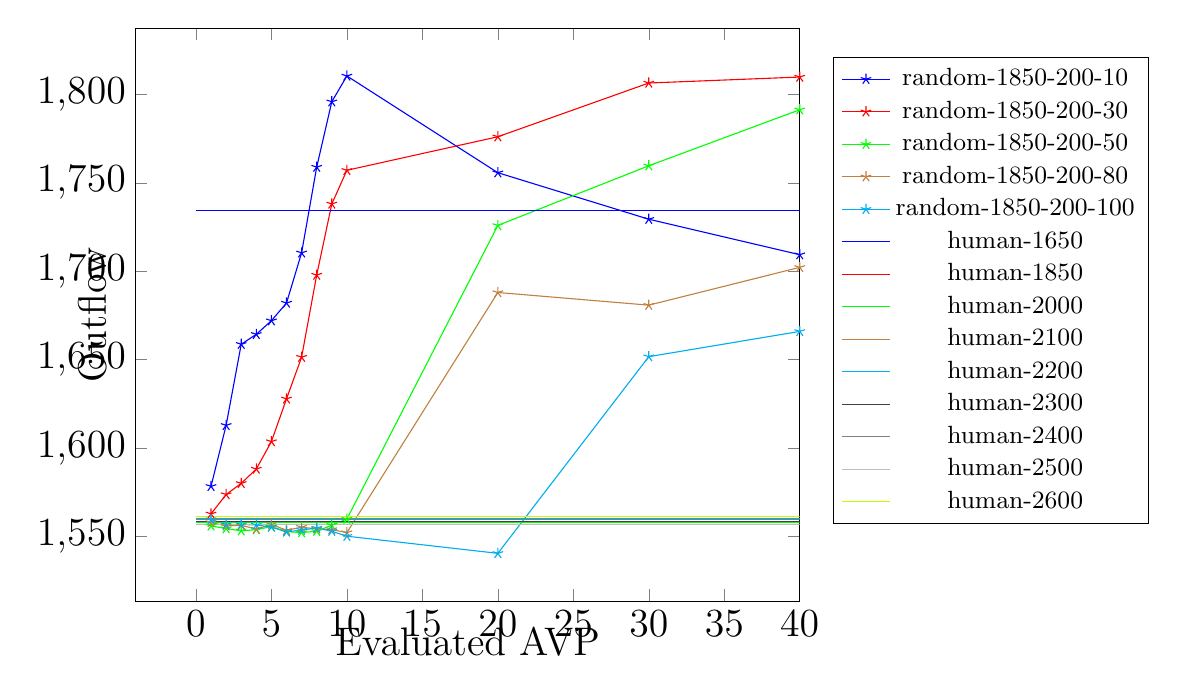
\begin{tikzpicture}[scale=1]
  \pgfplotsset{
      scale only axis,
      every x tick label/.append style={font=\Large},
      every y tick label/.append style={font=\Large},
	legend style={at={(1.05,0.95)},anchor=north west}
  }

\pgfplotscreateplotcyclelist{mycolorlist}{%
	 blue,  every mark/.append style={fill=blue!20}, mark=star, error bars/.cd, y dir=both, y explicit\\
	 red, densely dashed every mark/.append style={fill=red!20}, mark=star, error bars/.cd, y dir=both, y explicit\\
	 green, dashed every mark/.append style={fill=green!20}, mark=star, error bars/.cd, y dir=both, y explicit\\
	 brown, densely dotted every mark/.append style={fill=brown!20}, mark=star, error bars/.cd, y dir=both, y explicit\\
	 cyan, loosely dotted every mark/.append style={fill=cyan!20}, mark=star, error bars/.cd, y dir=both, y explicit\\
	 darkgray, loosely dashed every mark/.append style={fill=darkgray!20}, mark=star, error bars/.cd, y dir=both, y explicit\\
	 gray, densely dashdotted every mark/.append style={fill=gray!20}, mark=star, error bars/.cd, y dir=both, y explicit\\
	 lightgray, loosely dashdottted every mark/.append style={fill=lightgray!20}, mark=star, error bars/.cd, y dir=both, y explicit\\
	 lime,  every mark/.append style={fill=lime!20}, mark=star, error bars/.cd, y dir=both, y explicit\\
	 magenta, densely dashed every mark/.append style={fill=magenta!20}, mark=star, error bars/.cd, y dir=both, y explicit\\
	 olive, dashed every mark/.append style={fill=olive!20}, mark=star, error bars/.cd, y dir=both, y explicit\\
	 orange, densely dotted every mark/.append style={fill=orange!20}, mark=star, error bars/.cd, y dir=both, y explicit\\
	 pink, loosely dotted every mark/.append style={fill=pink!20}, mark=star, error bars/.cd, y dir=both, y explicit\\
	 purple, loosely dashed every mark/.append style={fill=purple!20}, mark=star, error bars/.cd, y dir=both, y explicit\\
	 teal, densely dashdotted every mark/.append style={fill=teal!20}, mark=star, error bars/.cd, y dir=both, y explicit\\
	 violet, loosely dashdottted every mark/.append style={fill=violet!20}, mark=star, error bars/.cd, y dir=both, y explicit\\
	 yellow,  every mark/.append style={fill=yellow!20}, mark=star, error bars/.cd, y dir=both, y explicit\\
	 Bittersweet, densely dashed every mark/.append style={fill=Bittersweet!20}, mark=star, error bars/.cd, y dir=both, y explicit\\
	 BlueViolet, dashed every mark/.append style={fill=BlueViolet!20}, mark=star, error bars/.cd, y dir=both, y explicit\\
	 BrickRed, densely dotted every mark/.append style={fill=BrickRed!20}, mark=star, error bars/.cd, y dir=both, y explicit\\
	 BurntOrange, loosely dotted every mark/.append style={fill=BurntOrange!20}, mark=star, error bars/.cd, y dir=both, y explicit\\
	 CadetBlue, loosely dashed every mark/.append style={fill=CadetBlue!20}, mark=star, error bars/.cd, y dir=both, y explicit\\
	 CarnationPink, densely dashdotted every mark/.append style={fill=CarnationPink!20}, mark=star, error bars/.cd, y dir=both, y explicit\\
	 Cerulean, loosely dashdottted every mark/.append style={fill=Cerulean!20}, mark=star, error bars/.cd, y dir=both, y explicit\\
	 Dandelion,  every mark/.append style={fill=Dandelion!20}, mark=star, error bars/.cd, y dir=both, y explicit\\
	 DarkOrchid, densely dashed every mark/.append style={fill=DarkOrchid!20}, mark=star, error bars/.cd, y dir=both, y explicit\\
	 Emerald, dashed every mark/.append style={fill=Emerald!20}, mark=star, error bars/.cd, y dir=both, y explicit\\
	 Fuchsia, densely dotted every mark/.append style={fill=Fuchsia!20}, mark=star, error bars/.cd, y dir=both, y explicit\\
	 GreenYellow, loosely dotted every mark/.append style={fill=GreenYellow!20}, mark=star, error bars/.cd, y dir=both, y explicit\\
	 Magenta, loosely dashed every mark/.append style={fill=Magenta!20}, mark=star, error bars/.cd, y dir=both, y explicit\\
	 Maroon, densely dashdotted every mark/.append style={fill=Maroon!20}, mark=star, error bars/.cd, y dir=both, y explicit\\
	 MidnightBlue, loosely dashdottted every mark/.append style={fill=MidnightBlue!20}, mark=star, error bars/.cd, y dir=both, y explicit\\
	 Orange,  every mark/.append style={fill=Orange!20}, mark=star, error bars/.cd, y dir=both, y explicit\\
	 OrangeRed, densely dashed every mark/.append style={fill=OrangeRed!20}, mark=star, error bars/.cd, y dir=both, y explicit\\
	 Orchid, dashed every mark/.append style={fill=Orchid!20}, mark=star, error bars/.cd, y dir=both, y explicit\\
	 Periwinkle, densely dotted every mark/.append style={fill=Periwinkle!20}, mark=star, error bars/.cd, y dir=both, y explicit\\
	 RawSienna, loosely dotted every mark/.append style={fill=RawSienna!20}, mark=star, error bars/.cd, y dir=both, y explicit\\
} %end of colors


\begin{axis}[
    legend style={font=\small},
	ylabel={\Large Outflow},
	x label style={at={(axis description cs:0.5,-0.03)},anchor=north},
	y label style={at={(axis description cs:-0.030,0.5)}, anchor=south},
	%xticklabel style = {font=\small,xshift=0.5ex},
	xlabel={\Large Evaluated AVP},
	legend columns=15,
	transpose legend,
	/tikz/column /.style={
                column sep=5pt,
            },
	cycle list name=mycolorlist,
	 xmax=40
]
%end of axis
\addplot table [x=a, y=b] {
a	 b	 c
1	1578.42	16.21
2	1612.91	18.97
3	1658.77	23.5
4	1664.39	21.81
5	1672.09	22.83
6	1682.1	23.34
7	1710.47	32.95
8	1758.96	33.62
9	1795.93	31.41
10	1810.51	28.73
20	1755.79	38.14
30	1729.48	36.16
40	1709.42	42.36
50	1687.46	35.91
60	1659.49	41.28
70	1622.38	54.02
80	1587.56	56.24
100	1531.69	56.26
};
\label{random-1850-200-10}

\addplot table [x=a, y=b] {
a	 b	 c
1	1562.83	15.83
2	1573.78	15.35
3	1580.08	17.19
4	1588.21	20.74
5	1603.73	18.79
6	1627.88	22.59
7	1651.46	26.07
8	1697.9	31.4
9	1738.12	27.42
10	1757.16	26.37
20	1776.13	47.77
30	1806.52	43.19
40	1809.9	41.44
50	1808.21	30.71
60	1803.71	33.3
70	1802.74	30.27
80	1791.32	25.59
100	1763.96	26.64
};
\label{random-1850-200-30}

\addplot table [x=a, y=b] {
a	 b	 c
1	1556.03	13.05
2	1554.52	14.18
3	1553.26	14.09
4	1553.9	13.38
5	1555.63	14.08
6	1552.79	15.65
7	1552.25	16.07
8	1553.04	16.82
9	1556.46	15.41
10	1559.92	16.29
20	1725.98	37.02
30	1759.72	53.04
40	1791.4	44.49
50	1814.94	38.71
60	1804.82	37.74
70	1803.92	31.76
80	1792.87	27.42
100	1759.93	27.77
};
\label{random-1850-200-50}

\addplot table [x=a, y=b] {
a	 b	 c
1	1557.97	14.18
2	1556.03	13.19
3	1556.32	13.31
4	1554.23	14.68
5	1556.86	15.02
6	1553.54	12.27
7	1555.31	14.88
8	1554.3	16.09
9	1553.98	14.08
10	1552.21	16.42
20	1688.04	24.67
30	1680.88	36.8
40	1702.26	50.61
50	1726.7	51.5
60	1761.34	56.24
70	1784.7	50.65
80	1794.53	40.4
100	1784.23	28.79
};
\label{random-1850-200-80}

\addplot table [x=a, y=b] {
a	 b	 c
1	1559.59	15.06
2	1556.82	12.66
3	1556.82	16.25
4	1556.57	14.51
5	1555.34	13.48
6	1552.64	14.58
7	1553.69	14.2
8	1554.84	14.1
9	1553.04	15.07
10	1550.2	14.54
20	1540.51	16.07
30	1651.75	28.07
40	1666.04	23.78
50	1659.56	30.07
60	1685.3	41.46
70	1739.95	47.67
80	1785.89	64.6
100	1797.19	26.94
};
\label{random-1850-200-100}

\addplot[blue, samples=200] coordinates {(0,1734.550000) (100,1734.550000)};\label{human-1650}\addplot[red, samples=200] coordinates {(0,1560.380000) (100,1560.380000)};\label{human-1850}\addplot[green, samples=200] coordinates {(0,1558.120000) (100,1558.120000)};\label{human-2000}\addplot[brown, samples=200] coordinates {(0,1560.310000) (100,1560.310000)};\label{human-2100}\addplot[cyan, samples=200] coordinates {(0,1560.380000) (100,1560.380000)};\label{human-2200}\addplot[darkgray, samples=200] coordinates {(0,1558.660000) (100,1558.660000)};\label{human-2300}\addplot[gray, samples=200] coordinates {(0,1559.520000) (100,1559.520000)};\label{human-2400}\addplot[lightgray, samples=200] coordinates {(0,1556.640000) (100,1556.640000)};\label{human-2500}\addplot[lime, samples=200] coordinates {(0,1561.280000) (100,1561.280000)};\label{human-2600}\addlegendimage{/pgfplots/refstyle=random-1850-200-10}
\addlegendentry{random-1850-200-10}
\addlegendimage{/pgfplots/refstyle=random-1850-200-30}
\addlegendentry{random-1850-200-30}
\addlegendimage{/pgfplots/refstyle=random-1850-200-50}
\addlegendentry{random-1850-200-50}
\addlegendimage{/pgfplots/refstyle=random-1850-200-80}
\addlegendentry{random-1850-200-80}
\addlegendimage{/pgfplots/refstyle=random-1850-200-100}
\addlegendentry{random-1850-200-100}
\addlegendimage{/pgfplots/refstyle=human-1650}
\addlegendentry{human-1650}
\addlegendimage{/pgfplots/refstyle=human-1850}
\addlegendentry{human-1850}
\addlegendimage{/pgfplots/refstyle=human-2000}
\addlegendentry{human-2000}
\addlegendimage{/pgfplots/refstyle=human-2100}
\addlegendentry{human-2100}
\addlegendimage{/pgfplots/refstyle=human-2200}
\addlegendentry{human-2200}
\addlegendimage{/pgfplots/refstyle=human-2300}
\addlegendentry{human-2300}
\addlegendimage{/pgfplots/refstyle=human-2400}
\addlegendentry{human-2400}
\addlegendimage{/pgfplots/refstyle=human-2500}
\addlegendentry{human-2500}
\addlegendimage{/pgfplots/refstyle=human-2600}
\addlegendentry{human-2600}


\end{axis}
\end{tikzpicture}
\end{document}
